\documentclass[11pt,a4paper]{article}
    \usepackage[margin=2.5cm]{geometry}
    \usepackage{enumitem}
    \usepackage{hyperref}
    \usepackage{tikz}
    \usetikzlibrary{arrows.meta,positioning,shapes.geometric}
    \title{Miscellaneous Utilities}
\author{Jordi Vill\`a-Freixa \texttt{<jordi.villa@uvic.cat>}}
    \date{\today}

    \tikzset{
      methodbox/.style={
        rounded corners=6pt,
        draw=blue!50!black,
        line width=0.9pt,
        fill=blue!6,
        minimum width=13cm,
        text width=11.8cm,
        align=left,
        inner sep=8pt
      }
    }

    \begin{document}
    \maketitle

    \section*{Scope}
    This folder combines general study resources with a small practical utility for collecting publication metadata from ORCID.

    \section*{Material in this folder}
    \begin{itemize}[leftmargin=*]
\item \texttt{retrievePublications.py}
\item \texttt{GitHubTricks.md}
    \end{itemize}

    \section*{Method summary}
    \begin{itemize}[leftmargin=*]
\item \textbf{ORCID publication harvesting}. The Python script queries the ORCID public API, extracts publication metadata, and filters records by year.
\item \textbf{DOI-based deduplication logic}. The retrieval workflow avoids duplicate output entries by using DOI fields as unique identifiers when available.
\item \textbf{Curated study references}. The markdown material serves as a curated pointer set for programming, statistics, and scientific work habits.
    \end{itemize}

    \section*{Method scheme}
    Figure~\ref{fig:summary} is drawn directly in LaTeX with TikZ. It is a compact conceptual map of the main workflows discussed in this folder.

    \begin{figure}[ht]
    \centering
    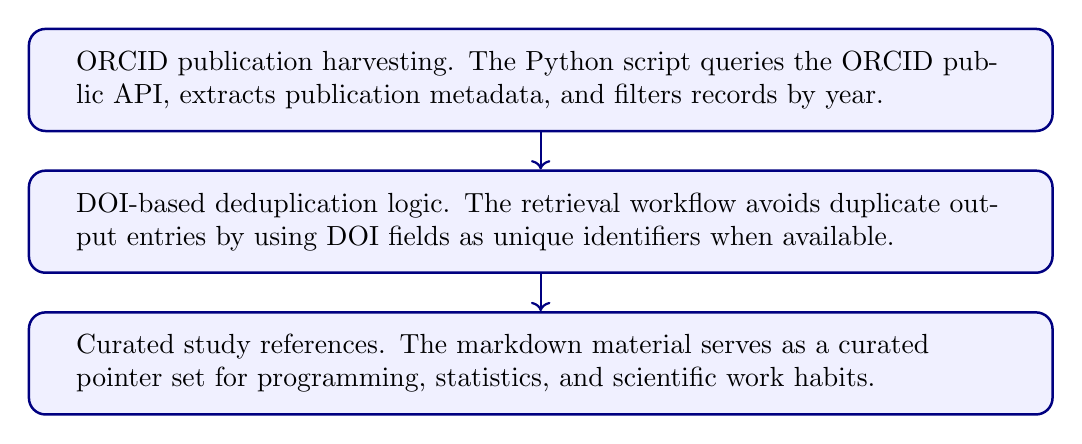
\begin{tikzpicture}[x=1cm,y=1cm]
    \node[methodbox] (m0) at (0,0.0) {ORCID publication harvesting. The Python script queries the ORCID public API, extracts publication metadata, and filters records by year.};
    \node[methodbox] (m1) at (0,-1.8) {DOI-based deduplication logic. The retrieval workflow avoids duplicate output entries by using DOI fields as unique identifiers when available.};
    \node[methodbox] (m2) at (0,-3.6) {Curated study references. The markdown material serves as a curated pointer set for programming, statistics, and scientific work habits.};
    \draw[->, thick, color=blue!50!black] (m0.south) -- (m1.north);
    \draw[->, thick, color=blue!50!black] (m1.south) -- (m2.north);
    \end{tikzpicture}
    \caption{Conceptual scheme for the methods in the miscellanea folder.}
    \label{fig:summary}
    \end{figure}

    
\section*{Disclaimer}
These documents were generated with the assistance of ChatGPT 5.4. The material has been reviewed by the author before inclusion in this repository, but it is not free from possible errors.

\end{document}